\documentclass[12pt,a4paper]{article}

\usepackage[utf8]{inputenc}
\usepackage[french]{babel}
\usepackage[T1]{fontenc}
\usepackage[margin=2cm]{geometry}
\usepackage{graphicx}
\usepackage{amsmath}
\usepackage{amsthm}
\usepackage{listings}
\usepackage{courier}

\lstset{basicstyle=\footnotesize\ttfamily,breaklines=true}
\lstset{framextopmargin=50pt,frame=bottomline}
\lstset{language=Scilab}

\usepackage{float}

\setlength{\parindent}{0pt}
\setlength{\parskip}{0.5em}

\title{\textbf{TP1 “MODÉLISER L’ALÉA” \\ CHAÎNES DE MARKOV CACHÉES}}
\author{Clément Riu - Louis Trezzini}
\date{24 avril 2017}

\newtheorem{lemme}{Lemme}

\begin{document}

\maketitle

\setcounter{section}{1}
\section{Crabes de Waldon}

\paragraph*{Question $1.$} On visualise l'histogramme des données ainsi que la gaussienne la plus proche afin d'évaluer si les données suivent une loi normale.

\begin{figure}[H]
	\centering
	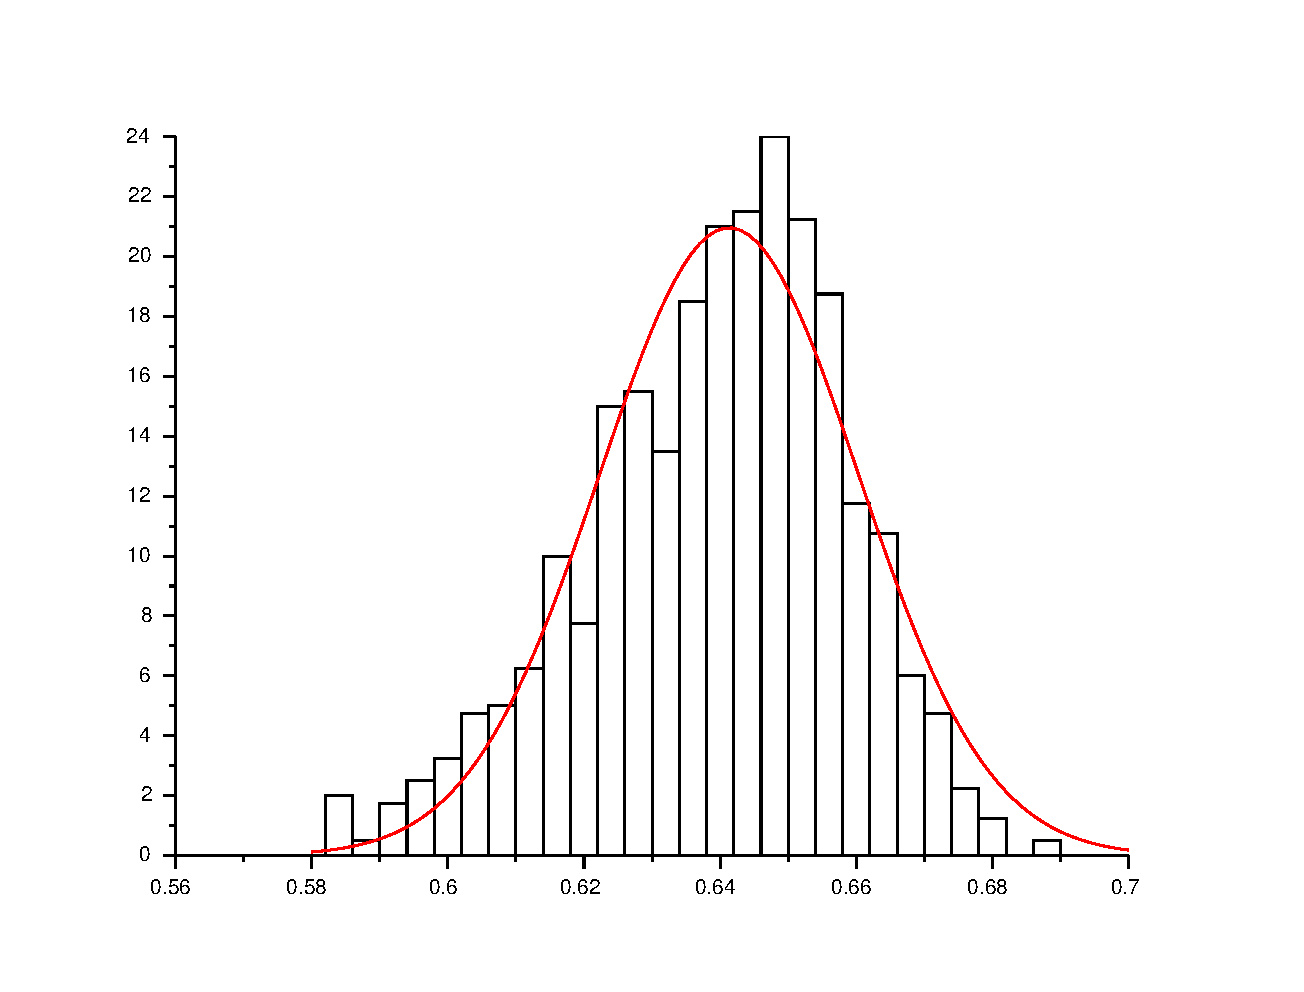
\includegraphics[width=0.95\textwidth]{images/figure0.eps}
	\caption{Loi empirique des données et gaussienne la plus proche.}
\end{figure}

Il y a un décallage entre la courbe théorique et les données empiriques, la loi normale n'explique pas bien les données.

\textit{Question subsidiaire $1.$} Lorsqu'on applique un test du $\chi^2$ aux données pour tester la normalité des données, le test est négatif : une loi normale ne permet pas d'expliquer les données.

\paragraph*{Question $2.$}

\paragraph*{Question $3.$} L'application de l'algorithme EM renvoie la courbe suivante :

\begin{figure}[H]
	\centering
	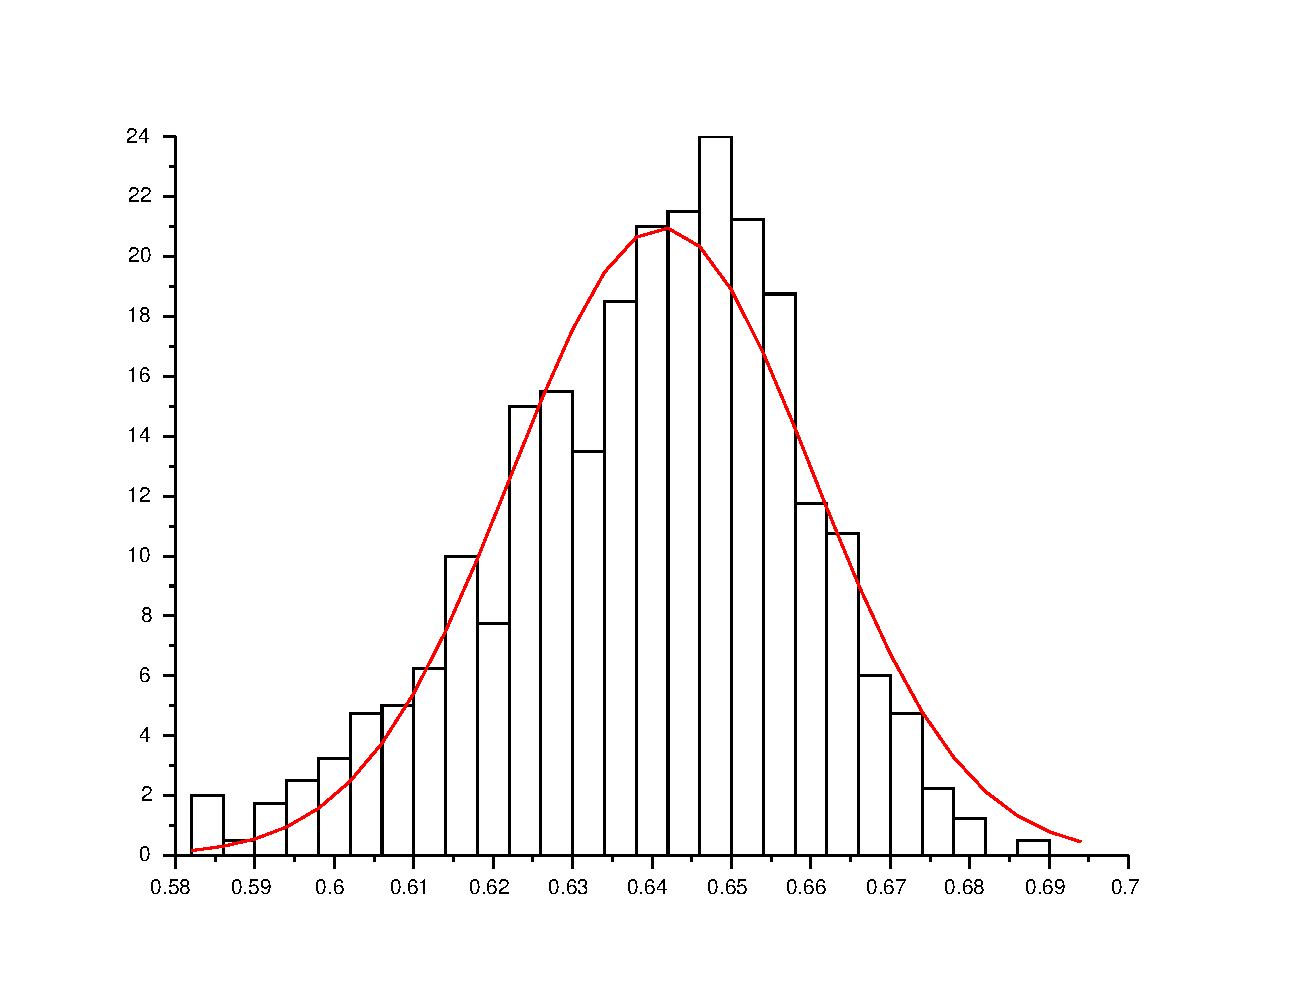
\includegraphics[width=0.95\textwidth]{images/figure1.eps}
	\caption{Loi empirique des données et les gaussiennes calculées par l'algorithme EM.}
\end{figure}

On remarque que la courbe en cyan suit bien les données empiriques, cette loi semble donc plus adéquate que la première proposition.

\textit{Question subsidiaire $2.$} On obtient dans le cas de $3$ populations le résultat suivant :

\begin{figure}[H]
	\centering
	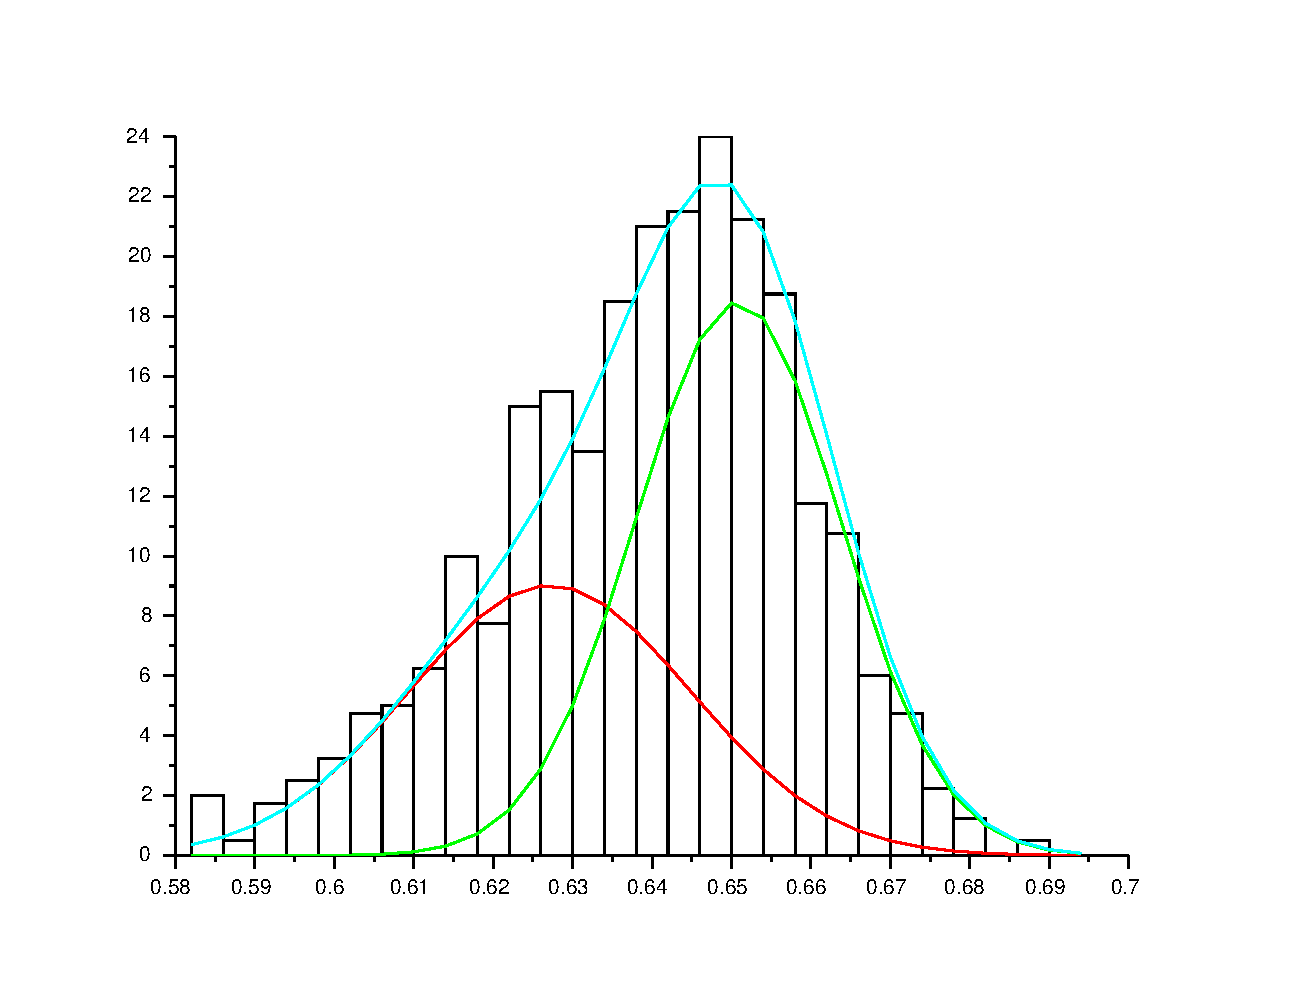
\includegraphics[width=0.95\textwidth]{images/figure2.eps}
	\caption{Loi empirique des données et les gaussiennes calculées par l'algorithme EM.}
\end{figure}

On observe que les crabes de faibles tailles font partis d'une population à part.

\section{Recherche de zones homogènes dans l'\textsc{ADN}}

\paragraph*{Question $4.$} On applique le calcul aux données restreintes avec les données initiales suivantes :

\begin{align*}
a &= \begin{pmatrix}
0.99 & 0.01 \\
0.03 & 0.97
\end{pmatrix} \\
b &= \begin{pmatrix}
0.2697410 & 0.2084444 & 0.1983422 & 0.3234723 \\
0.2463460 & 0.2475527 & 0.2982972 & 0.2078041
\end{pmatrix}\\
\pi_0 &= \begin{pmatrix}
0.5 \\
0.5
\end{pmatrix} \\
\end{align*}

On obtient alors les résultats finaux suivant :

\begin{align*}
a &= \begin{pmatrix}
0.9977068 & 0.0022932 \\
0 		  & 1
\end{pmatrix} \\
b &= \begin{pmatrix}
0.2576651 & 0.203861  & 0.2155776 & 0.3228962 \\  
0.1938853 & 0.2570135 & 0.3833224 & 0.1657789
\end{pmatrix}\\
\end{align*}

On observe alors les régions codantes et non-codantes :

\begin{figure}[H]
	\centering
	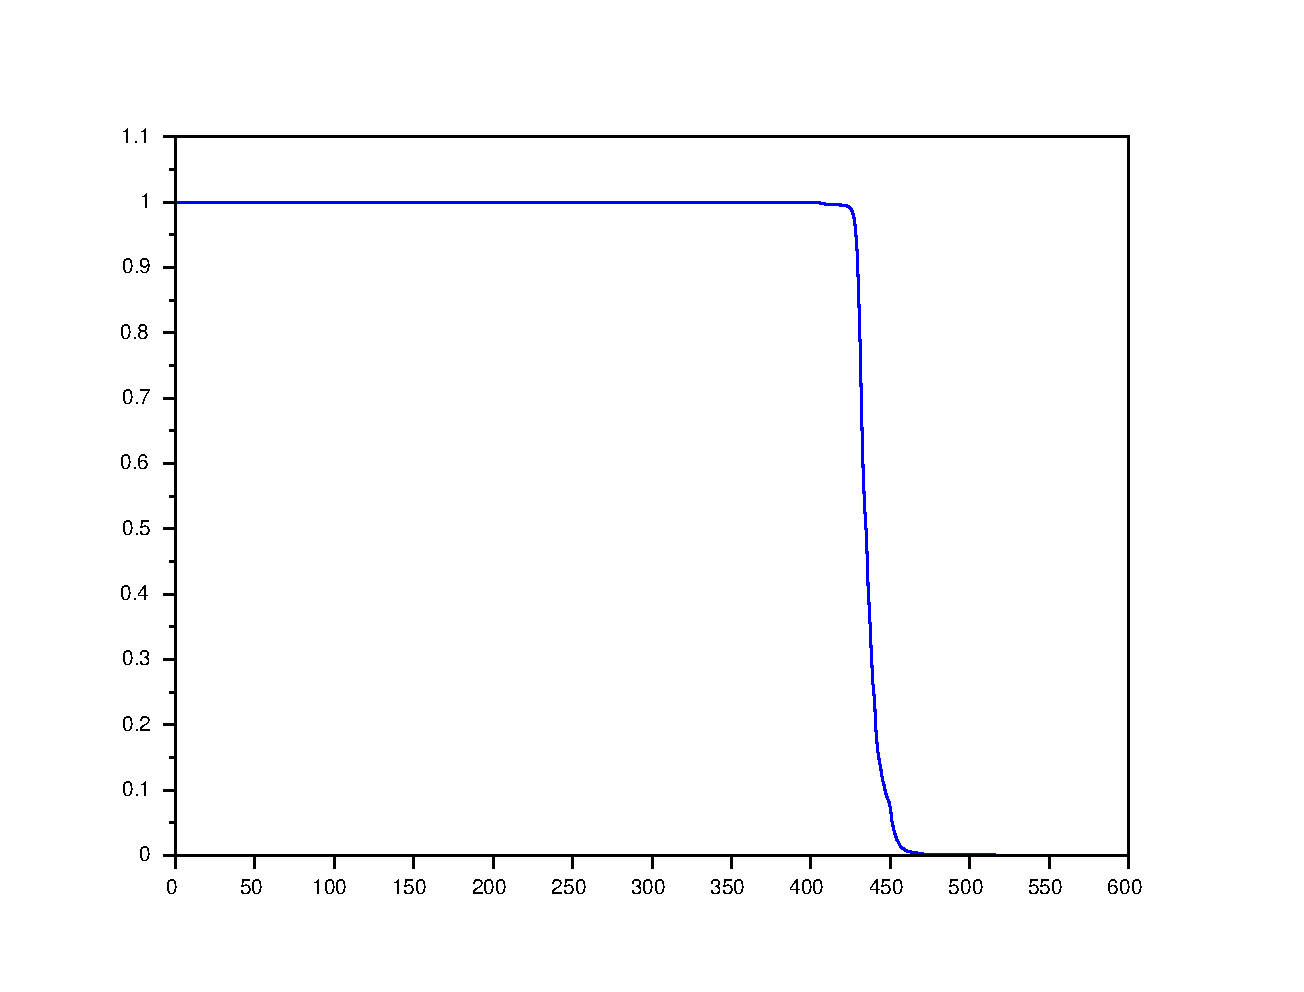
\includegraphics[width=0.95\textwidth]{images/figure3.eps}
	\caption{Les zone homogènes de la séquence d'\textsc{ADN}.}
\end{figure}

Les matrices $a$ et $b$ évoluent comme suit :

\begin{figure}[H]
	\centering
	\includegraphics[width=0.95\textwidth]{images/figure4.eps}\\
	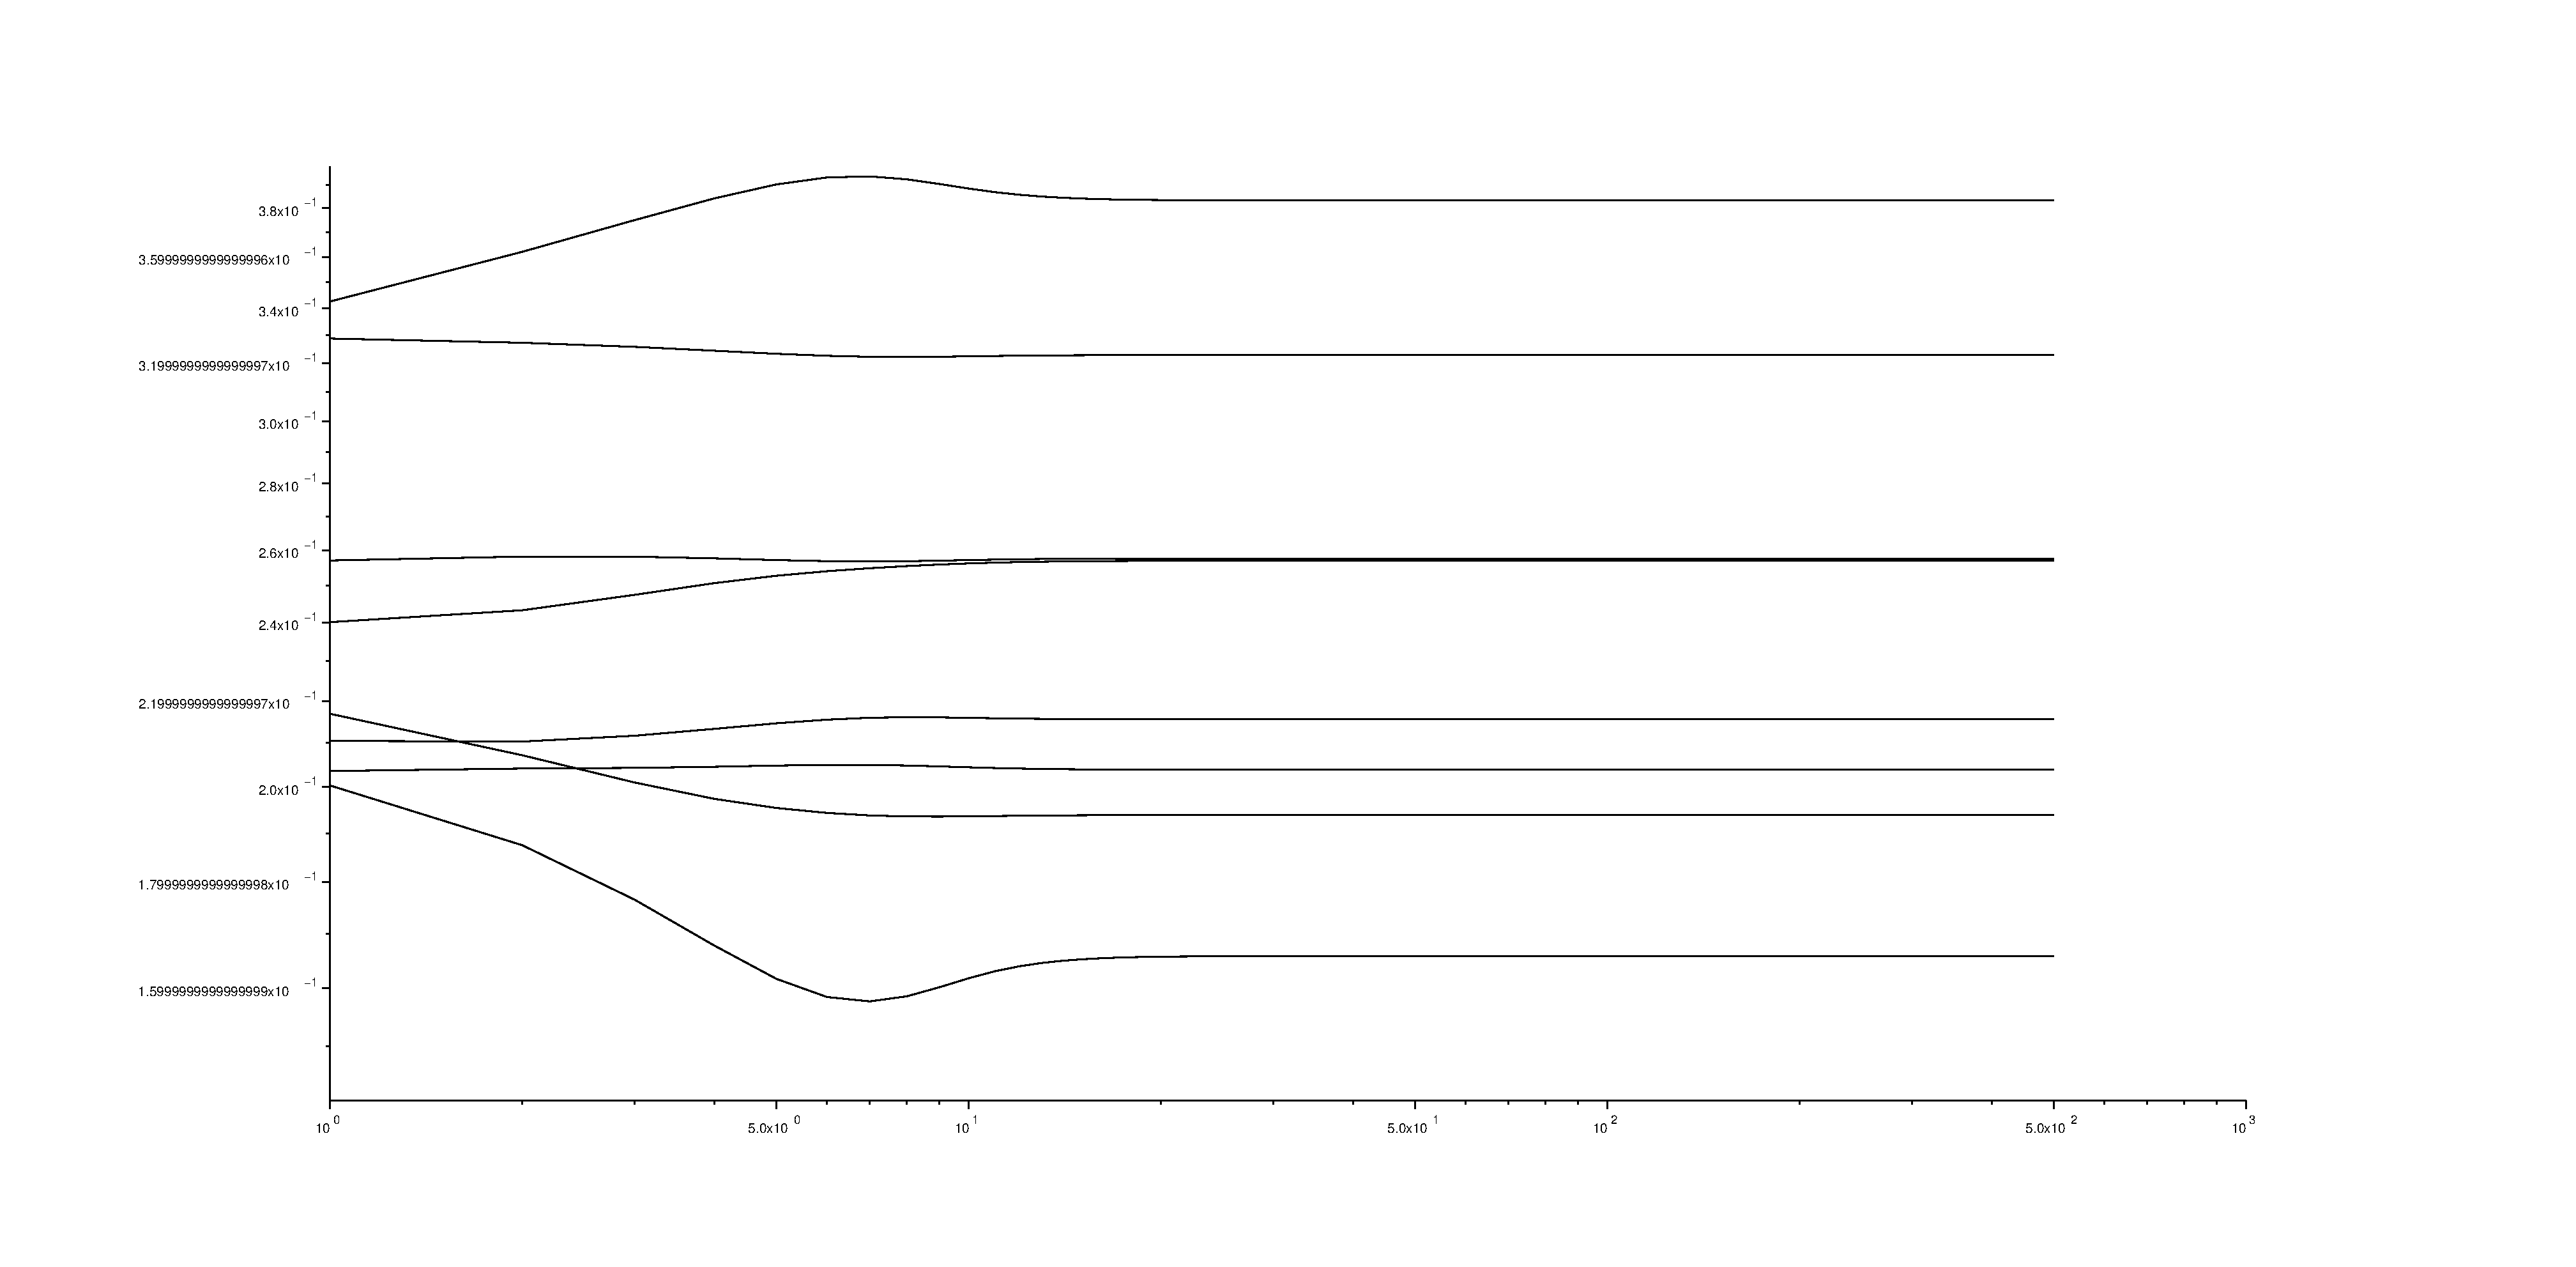
\includegraphics[width=0.95\textwidth]{images/figure5.eps}
	\caption{Évolution en échelle log-log des coefficients de la matrice $a$ (en haut) et de la matrice $b$ (en bas).}
\end{figure}

On remarque une convergence relativement rapide de l'algorithme, comme attendu d'après les résultats du livre \emph{Modèles aléatoires} de J.-F. Delmas et B. Jourdain.

Les données restreintes donnant des résultats satisfaisants, on observe le résultat sur la chaine complète :

\begin{figure}[H]
	\centering
	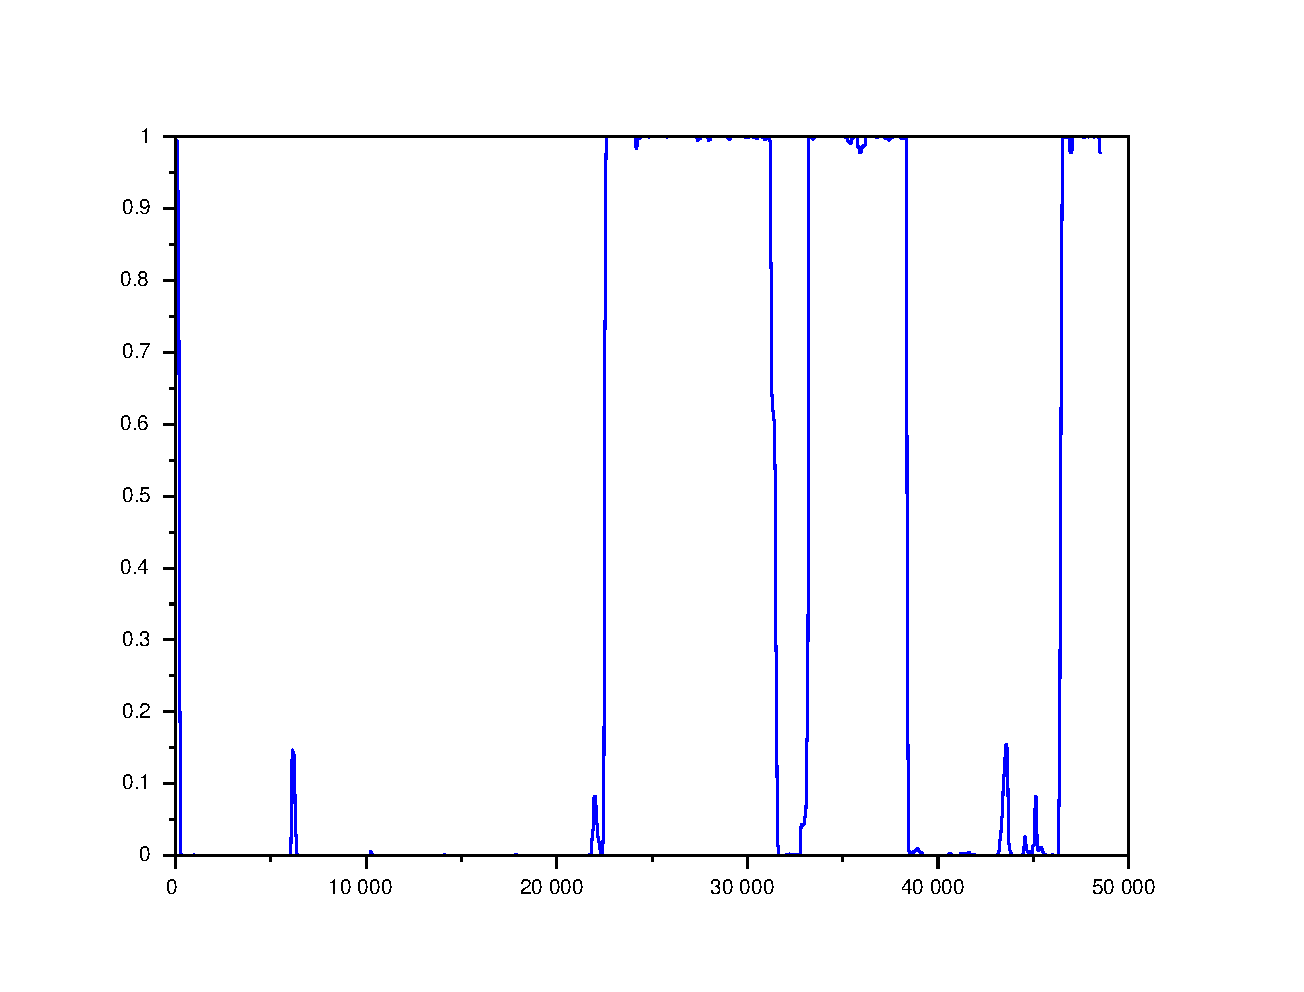
\includegraphics[width=0.95\textwidth]{images/figure6.eps}
	\caption{Les zone homogènes de la séquence d'\textsc{ADN}.}
\end{figure}
\begin{figure}[H]
	\centering
	\includegraphics[width=0.95\textwidth]{images/figure7.eps} \\
	\includegraphics[width=0.95\textwidth]{images/figure8.eps}
	\caption{Évolution en échelle log-log des coefficients de la matrice $a$ (en haut) et de la matrice $b$ (en bas).}
\end{figure}

En comparant aux résultat de la page $159$ on conclue que le résultat est satisfaisant.
\end{document}
